\chapter{研究方法}
\label{cha:experiment}

\section{应用功能设计}
\label{sec:app_design}
\begin{figure}[h]
	\centering
	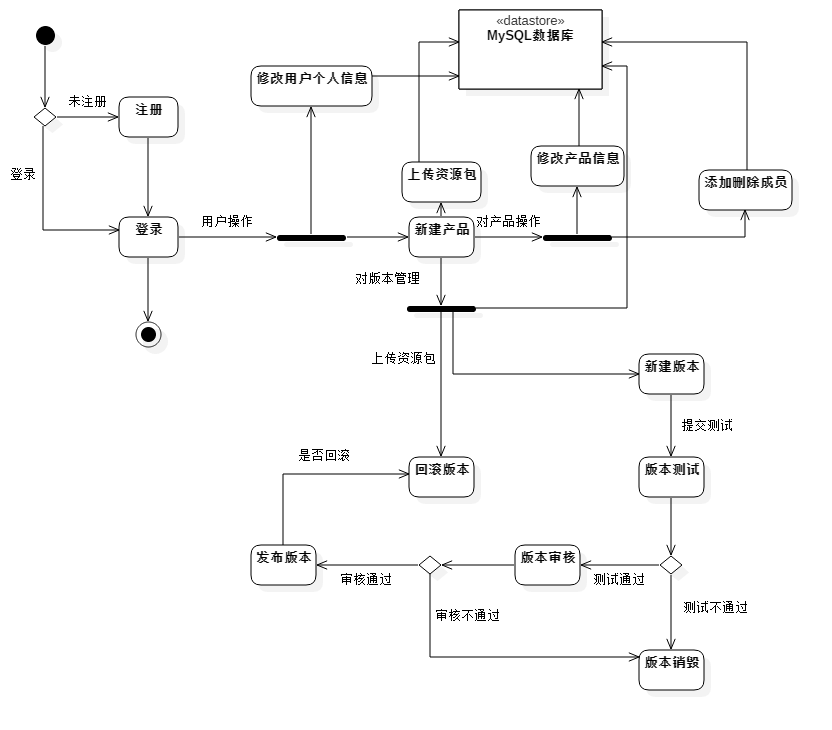
\includegraphics[width=0.8\textwidth]{image/UML/ActivityDiagram.png}
	\caption{应用功能设计}
	\label{fig:app}
\end{figure}
从上面的活动图可以看出,活动流程包含了三个方面:账户管理、产品管理(包括产品信息的修改和成员的增删)、对产品版本的管理
\begin{itemize}
	\item 账户的操作包括登录,注册,注销,更改个人信息
	\item 产品管理流程包括修改产品信息,修改(增删)产品成员信息
	\item 版本管理流程包括新建版本,版本从开发到发布的系列流程操控,版本回滚控制
\end{itemize}
\subsection{用户管理}
\label{sec:user}
账户的操作包括登录,注册,注销,更改个人信息
\subsection{产品管理}
\label{sec:product}
产品管理流程包括修改产品信息,修改(增删)产品成员信息
\subsection{版本管理}
\label{sec:version}
版本管理流程包括新建版本,版本从开发到发布的系列流程操控,版本回滚控制
\begin{figure}[h]
	\centering
	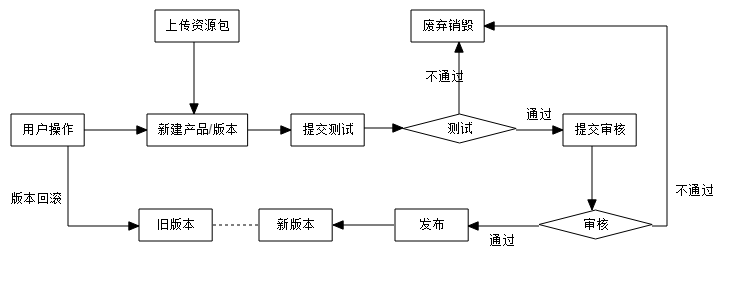
\includegraphics[width=0.8\textwidth]{image/UML/FlowchartDiagram.png}
	\caption{版本管理流程}
	\label{fig:version}
\end{figure}
\subsubsection{文件上传功能}
\label{sec:fileUpload}
\section{前端架构}
\label{sec:Front-end_architecture}
\begin{figure}[h]
	\centering
	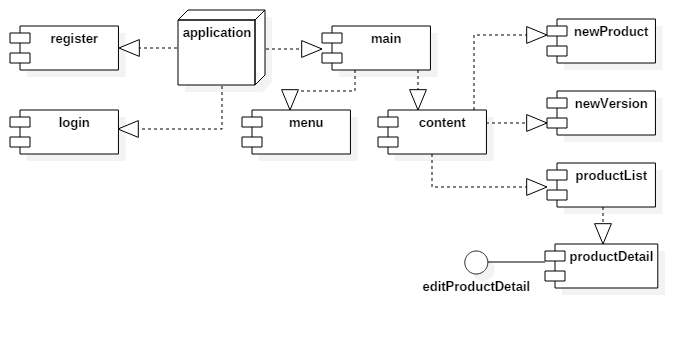
\includegraphics[width=0.8\textwidth]{image/UML/ComponentDiagram.png}
	\caption{前端架构}
	\label{fig:frame}
\end{figure}
angular的优点是模块化和组件化,将每个页面封装成一个个组件,利用路由功能在不同的组件之间跳跃,实现页面的快速跳转。
同时,利用模板语法和数据绑定,使得前后端开发分离,我们只需要从后台获得关键数据,即可在前台的HTML模板中填入数据,渲染页面	
\section{界面设计}
\label{sec:UI}
阿里巴巴针对angular封装了对应的UI风格和许多实用的组件供开发者使用,让开发者不必花费过多的时间在UI的设计上面,让开发的周期变得更短。

使用方法:npm install ng-zorro-antd
\section{数据库设计}
\label{sec:database_design}
本应用使用MySQL数据库建立一系列相互联系的表。之所以如此选择,一是因为本应用的各表之间的联系比较紧密,需要经常在多表之间进行联合查询,
二是MySQL支持事务功能,对数据进行CRUD的时候能保持原子性。
\begin{figure}[h]
	\centering
	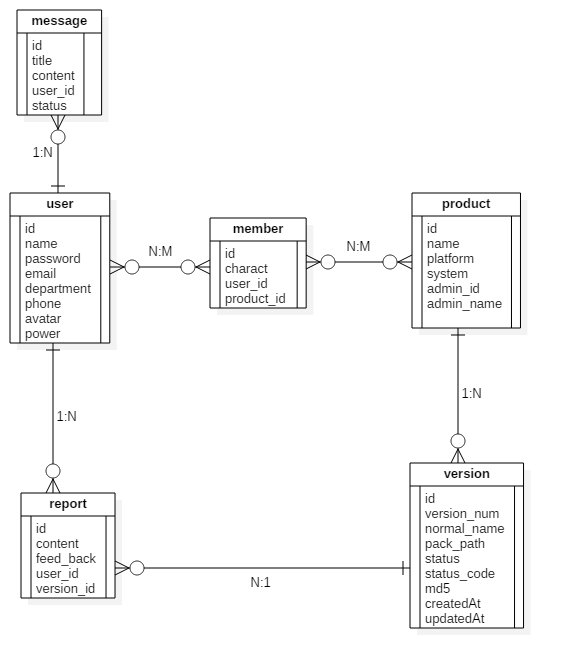
\includegraphics[width=0.8\textwidth]{image/UML/ERDDiagram.png}
	\caption{数据库设计}
	\label{fig:database}
\end{figure}
\section{后端开发}
\label{sec:Backend_development }
后端服务器采用express+nodejs进行搭建。用express可以快速搭建一个基于nodejs的服务器,我们只需要把精力都放在接口实现上即可。
将接口分门别类在对应的不同文件中,利用express的路由功能可以精确访问到接口。
而要使服务器能连接数据库,我们需要额外的模块,我们可以使用基于nodejs的mysql模块,
但是有一个热门的orm(Object Relationship Model)框架Sequelize对于描述表之间的关系,以及多表查询方面有更加好的解决方案,
同时Sequelize基于Promise实现异步流程控制,能更好地解决nodejs中数据库操作的回调地狱问题,
能够更方便我们对数据库进行操作,因此我们选用Sequelize来对数据库进行操作。